%!TEX root = ../report.tex
\section{Results}

\subsection{Model comparison}

\autoref{tab:performance} shows the performance of the different models on the test set after the hyperparameter tuning.
Even if it's not the most performing model, we choose the \gls{lr} as final model for its interpretability and simplicity, at the cost of just one percentage point in performance with respect to the \gls{rf}.

\autoref{fig:roc-comparison} shows the \gls{roc} curves of all the models.

\begin{table}
\centering
\caption{Comparison of performance.}
\label{tab:performance}
\begin{tabular}{lr}
\toprule
                 Model &    AUC \\
\midrule
RandomForestClassifier & 0.6769 \\
    LogisticRegression & 0.6702 \\
            GaussianNB & 0.6452 \\
DecisionTreeClassifier & 0.5943 \\
  KNeighborsClassifier & 0.5681 \\
         MLPClassifier & 0.5028 \\
\bottomrule
\end{tabular}
\end{table}


\begin{figure}[htpb]
    \centering
    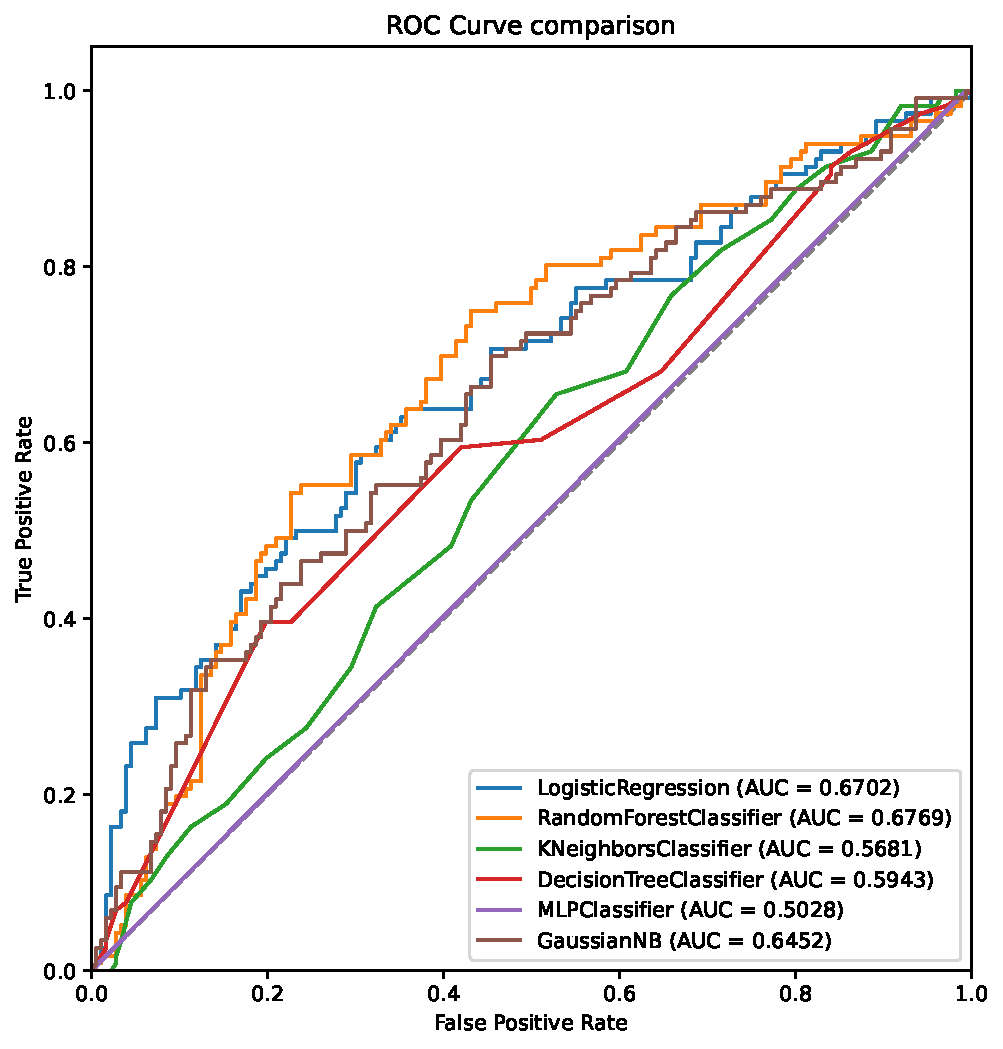
\includegraphics[width=3.1in]{roc_comparison.pdf}
    \caption{\gls{roc} curves comparison.}
    \label{fig:roc-comparison}
\end{figure}

% \subsection{Cross-validation inspection}

% \autoref{fig:crossvalidation_curve} shows the evolution of the CV for the final model.

% \begin{figure}[htpb]
%     \centering
%     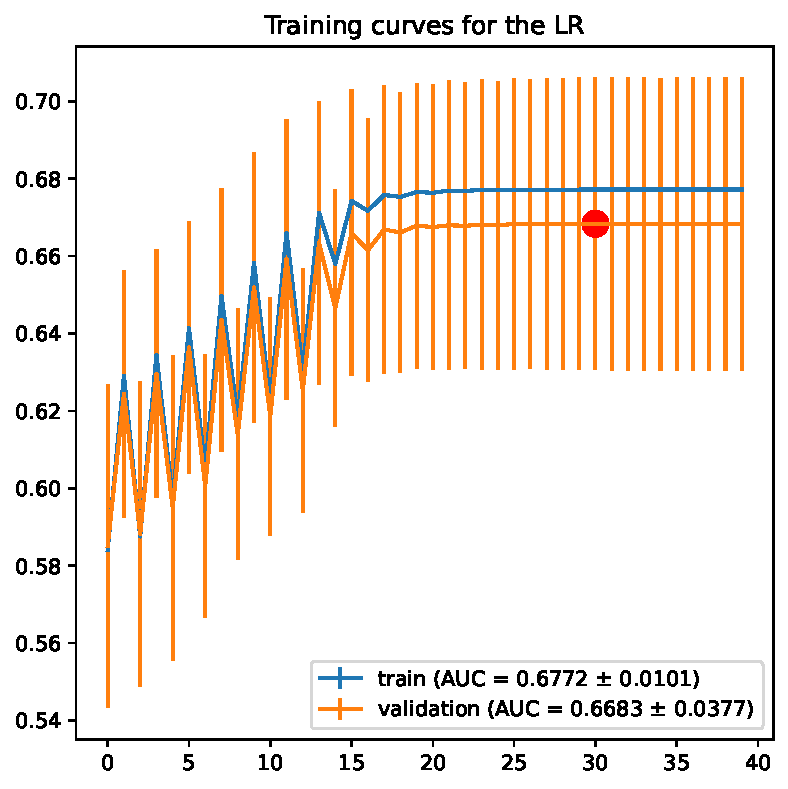
\includegraphics[width=3.1in]{crossvalidation_curve.pdf}
%     \caption{Training evolution.}
%     \label{fig:crossvalidation_curve}
% \end{figure}

\subsection{Model analysis}

Given a vector of variables $\bm{X} = X_1, \dots, X_p$ the \gls{lr} model assumes the following relationship between the variables and a prediction score $p(\bm{X})$, where $\beta_0, \beta_1, \dots, \beta_p$ are unknown real coefficients to be numerically estimated.
\begin{align*}
    \operatorname{logit}(p(\bm{X})) &= \log (\operatorname{odds}(p(\bm{X}))) = \log \left( \frac{p(\bm{X})}{1-p(\bm{X})} \right)\\
    & = \beta_0 + \beta_1 X_1 + \cdots + \beta_p X_p
\end{align*}
% Where the odds are therefore
% \begin{align*}
%     \operatorname{odds}p(\bm{X}) = \frac{p(\bm{X})}{1-p(\bm{X})} = e^{\beta_0 + \beta_1 X_1 + \cdots + \beta_p X_p}
% \end{align*}
% One can easily find the inverse relation
% \begin{align*}
%     p(\bm{X}) &= \frac{\exp(\beta_0 + \beta_1 X_1 + \cdots + \beta_p X_p)}{1+\exp(\beta_0 + \beta_1 X_1 + \cdots + \beta_p X_p)}
% \end{align*}
We can give an interpretation to the coefficients: if $\bm{1}_i$ is a vector of all zeros, and with a $1$ in $i$-th position:
\begin{align*}
\operatorname{OR}_i &= \frac{\operatorname{odds}(\bm{X}+\bm{1}_i)}{\operatorname{odds}(\bm{X})} = \frac{\left(\frac{p(\bm{X}+\bm{1}_i)}{1 - p(\bm{X}+\bm{1}_i)}\right)}{\left(\frac{p(\bm{X})}{1 - p(\bm{X})}\right)}\\
&= \frac{e^{\beta_0 + \beta_1 X_1 + \cdots + \beta_i (X_i + 1) + \cdots + \beta_p X_p}}{e^{\beta_0 + \beta_1 X_1 + \cdots + \beta_i X_i + \cdots + \beta_p X_p}} = e^{\beta_i}
\end{align*}
The odds multiply by $e^{\beta_i}$ for every 1-unit increase in $X_i$.
% 
% However, since we scaled the numerical data before fitting the model, the coefficient is intended for a 1-unit increase in the \emph{scaled} variable, but with some manipulation we can retrieve the effect for the original variable.
% \begin{align*}
% \operatorname{OR}_i = \frac{e^{\beta_i (\frac{(X_i+1)-\mu}{\sigma})}}{e^{\beta_i \frac{X_i-\mu}{\sigma}}} = e^{\frac{\beta_i}{\sigma}}
% \end{align*}

%In \autoref{fig:feature-importance-logistic-regression} we have the coefficients of the \gls{lr} for visualizing importance
In \autoref{tab:lr-coeff} we report the $\beta_i$ coefficients for the final model, together with $e^{\beta_i}$.

% \begin{figure}[htpb]
%     \centering
%     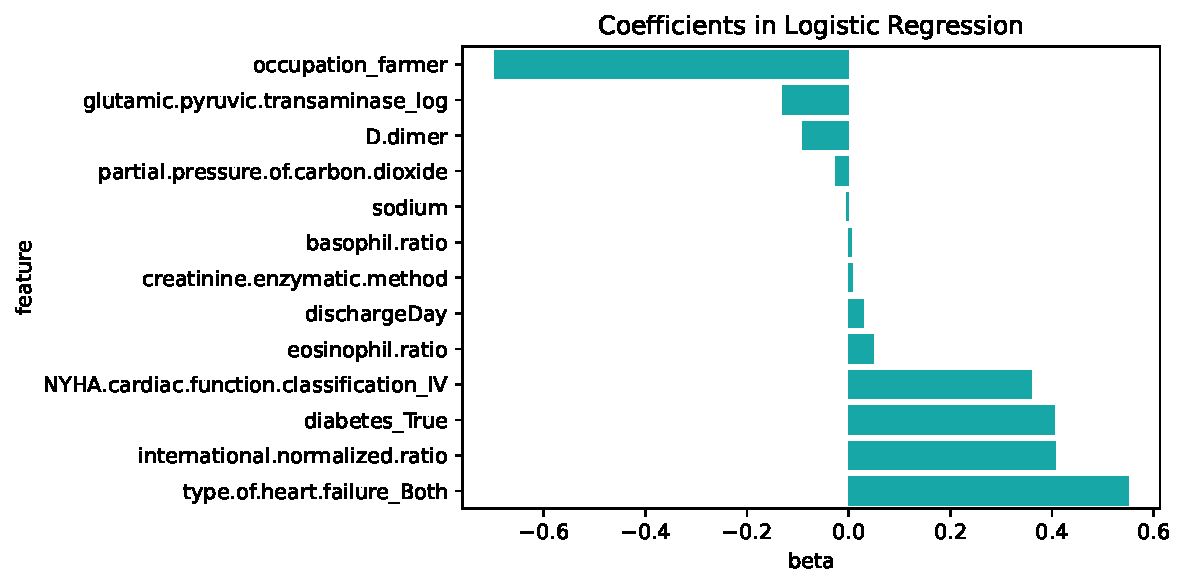
\includegraphics[width=3.1in]{feature_importance_weightsLogisticRegression.pdf}
%     \caption{Coefficients of the \gls{lr}.}
%     \label{fig:feature-importance-logistic-regression}
% \end{figure}

\begin{table}
\centering
\caption{Logistic Regression coefficients.}
\label{tab:lr-coeff}
\begin{tabular}{lrr}
\toprule
                                feature &    beta &  exp\_beta \\
\midrule
                      occupation\_farmer & -0.6973 &    0.4979 \\
      glutamic.pyruvic.transaminase\_log & -0.1305 &    0.8776 \\
                                D.dimer & -0.0911 &    0.9129 \\
     partial.pressure.of.carbon.dioxide & -0.0261 &    0.9743 \\
                                 sodium & -0.0049 &    0.9951 \\
                         basophil.ratio &  0.0055 &    1.0055 \\
            creatinine.enzymatic.method &  0.0066 &    1.0066 \\
                           dischargeDay &  0.0294 &    1.0298 \\
                       eosinophil.ratio &  0.0486 &    1.0498 \\
NYHA.cardiac.function.classification\_IV &  0.3599 &    1.4332 \\
                          diabetes\_True &  0.4049 &    1.4991 \\
         international.normalized.ratio &  0.4074 &    1.5029 \\
             type.of.heart.failure\_Both &  0.5502 &    1.7336 \\
\bottomrule
\end{tabular}
\end{table}


\subsection{Performance evaluation}

The confusion matrix produced by the \gls{lr} obtained with the default 0.5 threshold of Scikit-learn can be seen in \autoref{fig:confusion}, while \autoref{tab:classification-report} contains all the classification metrics. The Accuracy is 0.6370.

\begin{figure}[htpb]
\centering
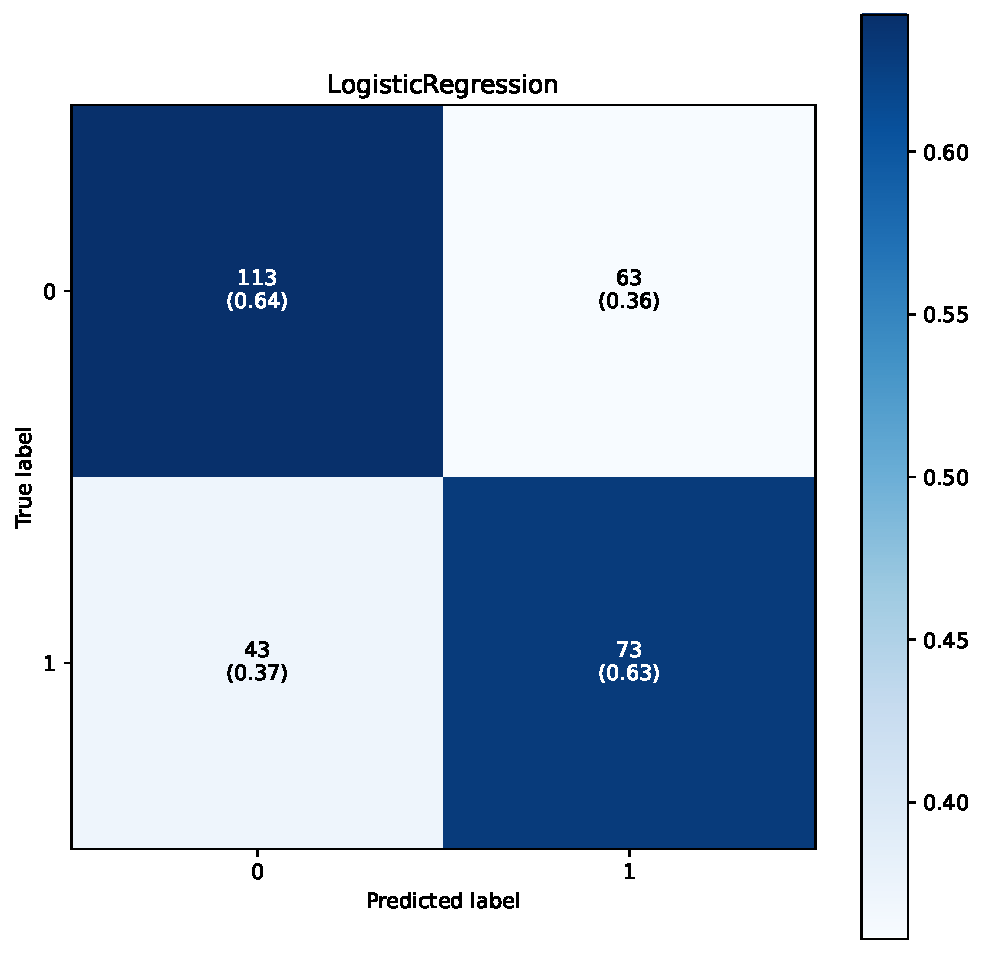
\includegraphics[width=3.1in]{confusion_matrix_LR.pdf}
\caption{Normalized confusion matrix.}
\label{fig:confusion}
\end{figure}

\begin{table}
\centering
\caption{Classification Report.}
\label{tab:classification-report}
\begin{tabular}{rrrr}
\toprule
 precision &  recall &  f1-score &  support \\
\midrule
    0.7244 &  0.6420 &    0.6807 &      176 \\
    0.5368 &  0.6293 &    0.5794 &      116 \\
    0.6306 &  0.6357 &    0.6300 &      292 \\
    0.6498 &  0.6370 &    0.6405 &      292 \\
\bottomrule
\end{tabular}
\end{table}


\subsection{Web App}

Trying to address the needs of clinicians who need user friendly tools to put our statistical results into practice, we developed a web app using the Python library \texttt{streamlit}, to easily input values and get predictions from our final model.

The web app is accessible through the following link:
\url{https://teobucci-slhd-app-3iahgf.streamlit.app/}
